\newpage

\section{Internal Software}

The in this section described processes are internal processes, i.e. running on the robot itself. In total there are three custom processes running on the robot. Figure \ref{fig:software} shows the structure of the developed software. This section focuses on the base and the navigation process. The image streaming process is referenced in section \ref{sec:image_processing}.

\begin{figure}[H]
\centering
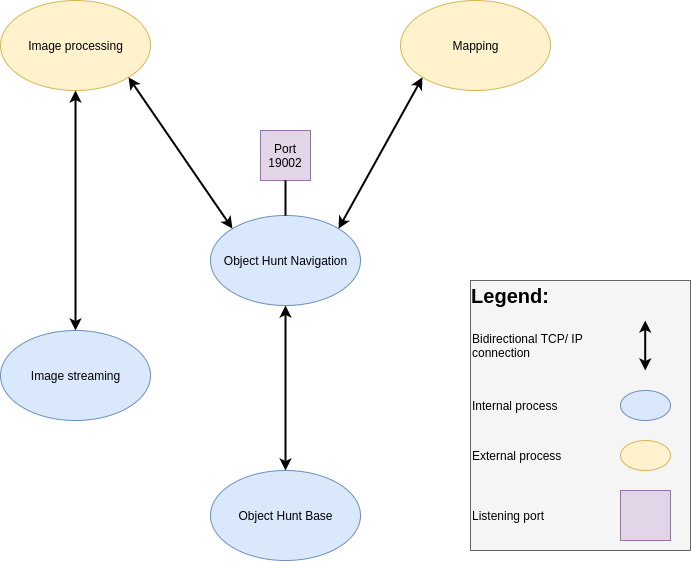
\includegraphics[scale=0.6]{sources/software_structure.png}
\caption[Software structure]{Software structure}
\label{fig:software}
\end{figure}

\subsection{Design Principles}

The internal software underlies software specifications, which are defined at the beginning of the project. They define among other things how the system as a whole will behave and handle dedicated tasks, i.e. communication. The compliance of these principles ensure that the developed software works in the expected manner and offers the possibility for adding further processes in the future.

\begin{itemize}
\itemsep0em
\item Communication
	\begin{itemize}
	\item Via TCP/\,IP
	\item Independent from other devices
	\item Beyond system border
	\end{itemize}
	
\item Economical
	\begin{itemize}
	\item No unnecessary CPU consume
	\item Fast reaction times
	\item Event driven
	\end{itemize}
	
\item Documentation
	\begin{itemize}
	\item Complete
	\item Easy accessible
	\end{itemize}
\end{itemize}

\subsection{Base Process}

\subsection{Navigation Process}


